\documentclass{article}
\usepackage{amsfonts}          % Para las negrita de pizarra
\usepackage{indentfirst}       % Para que quede mas lindo el formateo
\usepackage{graphicx}          % Para graficos
\usepackage{minted}            % Para poner codigo y que quede con sintaxis fachera
\usepackage{hyperref}          % Para meter hipervinculos
\usepackage[dvipsnames]{xcolor}% Para usar colores
\usepackage{hhline}            % Mas configuracion para las líneas en tablas
\usepackage{amsmath}           % Agregado para tags de ecuaciones
\usepackage{xcolor}            % Coloreado de ecuaciones
\usepackage{quoting, xparse}   % Usado para citar
% \usepackage{svg}               % Para usar imagenes svg que se ven lindas independientemente del zoom. WARNING REQUIERE DE INKSCAPE. Tal vez no vale la pena
\usepackage{amsmath}           % Configuraciones adicionales a las ecuaciones (creo)

\setcounter{tocdepth}{4}       %\
                               % > Hace que \paragraph aparezca en el TOC
\setcounter{secnumdepth}{4}    %/

\graphicspath{ {./images/} }

\newcommand{\docuPy}{%
  {\href{https://wiki.python.org/moin/TimeComplexity}{documentación oficial}}
  }%

  % Comandos para facilitar el citado
  % Fuente: https://tex.stackexchange.com/a/391739/273865
\NewDocumentCommand{\bywhom}{m}{% the Bourbaki trick
  {\nobreak\hfill\penalty50\hskip1em\null\nobreak
   \hfill\mbox{\normalfont(#1)}%
   \parfillskip=0pt \finalhyphendemerits=0 \par}%
}

\begin{document}

\begin{titlepage}
  \vspace*{1cm}

  \begin{center}
    {\Huge{Trabajo Práctico 3: Problemas NP-Completos para la defensa de la Tribu del Agua}}
  \end{center}

  \vspace{0.4cm}

  \begin{center}
    {\LARGE{Facultad de Ingeniería de la Universidad de Buenos Aires}}\\
    \vspace{0.3cm}
    {\Large{Teoría de Algoritmos}}\\
    \vspace{0.3cm}
    {\large{Cátedra Buchwald-Genender}}\\
  \end{center}

  \vspace{0.8cm}
  \begin{center}
    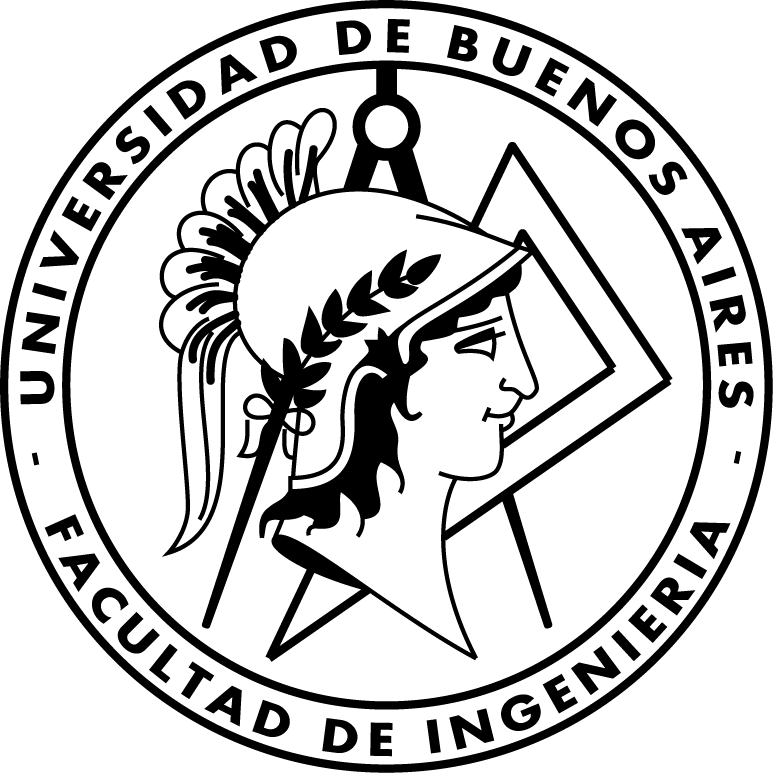
\includegraphics[scale=0.8]{Logo-fiuba}
  \end{center}

  \vspace{1.4cm}
  \begin{center}

    {\begin{minipage}[t]{.32\textwidth}
        \begin{center}
          Gómez Belis, Sofía\\
          {\small{Padrón: 109358}}\\
          {\small{email: sgomezb@fi.uba.ar}}
        \end{center}
          \end{minipage}
          \begin{minipage}[t]{.32\textwidth}
        \begin{center}
          Llanos Pontaut, Valentina\\
          {\small{Padrón: 104413}}\\
          {\small{email: vllanos@fi.uba.ar}}\\
        \end{center}
      \end{minipage}
      \begin{minipage}[t]{.32\textwidth}
        \begin{center}
          Orsi, Tomas Fabrizio\\
          {\small{Padrón: 109735}}\\
          {\small{email: torsi@fi.uba.ar}}
        \end{center}
      \end{minipage}}

  \end{center}
\end{titlepage}

\renewcommand*\contentsname{Indice}
\tableofcontents
\pagebreak

\section{Introducción}
\subsection{Descripción y objetivo}
\label{sec:descripcion}

Continuando con el ataque de la Nación del Fuego sobre el resto de las naciones, esta vez es la Tribu del Agua la que requiere de nuestra ayuda para defenderse. 

Cada maestro agua tiene una fuerza o habilidad positiva $x_i$, y contamos con el conjunto de todos los valores $(x_i, x_2, \dots, x_n)$. Basándonos en estos, el maestro Pakku desea separar los maestros en \texttt{k} grupos $(S_1, S_2, \dots, S_k)$ parejos tal que cuando un grupo se canse, entrará el siguiente en el combate, obteniendo un ataque constante que les permita salir victoriosos, aprovechando también la ventaja del agua por sobre el fuego.

Para que los grupos estén lo más parejos posibles, nos han encomendado minimizar la adición de los cuadrados de las sumas de las fuerzas de los grupos:

$$
\min \sum_{i=1}^{k} \left( \sum_{x_j \in S_i} x_j \right)^2
$$

En este trabajo desarrollaremos algoritmos de backtracking, programación lineal y posibles aproximaciones buscando resolver el problema de optimización planteado con el objetivo de ayudar a los mestros de la Tribu del Agua a derrotar a la Nación del Fuego. También nos dedicaremos a demostrar que el problema de la tribu del agua es NP-Completo.

\section{Demostración de problema NP-Completo}
\label{sec:np-completo}

Los problemas NP-Completos son los problemas más difíciles de NP. Cualquier problema en NP puede ser reducido a uno NP-Completo.

Para demostrar que el problema de la Tribu del Agua es NP-Completo, primero debemos demostrar que se encuentra en NP. Posteriormente, si logramos hacer una reducción polinomial de un problema NP-Completo a éste, entonces esto implica que también se trata de un problema NP-Completo. Ésto se debe a que la reducción $Y \leq_p X$ implica que la dificultad de resolver \texttt{Y} se reduce polinomialmente a la dificultad de resolver \texttt{X}, o que \texttt{X} es al menos tan difícil de resolver como \texttt{Y}. Si \texttt{Y} es un problema NP-Completo, entonces \texttt{X} es al menos tan difícil de resolver como un problema NP-Completo.

Para realizar la demostración y la reducción, necesitamos basarnos en el problema de decisión:

Dados una secuencia de \texttt{n} fuerzas de maestros agua $(x_i, x_2, \dots, x_n)$, y dos números \texttt{k} y \texttt{B}, ¿existe una partición en \texttt{k} subgrupos $(S_1, S_2, \dots, S_k)$ tal que:

$$
\sum_{i=1}^{k} \left( \sum_{x_j \in S_i} x_j \right)^2 \leq B
$$

y cada elemento $x_i$ esté asignado a solamente un grupo?
\subsection{Problema en NP}
\label{sec:taEnNp}

Un problema se encuentra en NP si existe un certificador eficiente para el mismo. Es decir, si puede ser verificado o validado en tiempo polinomial. 

Tenemos los siguientes datos:
\begin{itemize}
    \item Habilidades de los maestros $\rightarrow$ se presentan en forma de tupla (nombre maestro, fuerza)
    \item Cantidad de subconjuntos $\rightarrow$ \texttt{k}
    \item Cota del coeficiente $\rightarrow$ \texttt{B}
    \item Resultado a validar $\rightarrow$ subconjuntos $S_i$ que contienen los nombres de los maestros del grupo correspondiente
\end{itemize}

También tenemos las siguientes restricciones:
\begin{itemize}
    \item Cada maestro debe estar asignado a un solo grupo
    \item El resultado debe contener \texttt{k} grupos
    \item La sumatoria resultante debe ser a lo sumo \texttt{B} 
\end{itemize}

Dados estos datos y restricciones, proponemos el siguiente certificador.
\inputminted[linenos, firstline=1, lastline=31]{python}{codigo/certificador_eficiente.py}

Para que el verificador presentado pueda ser considerado un certificador eficiente, debe ejecutarse en tiempo polinomial. Por lo tanto, procedemos a explicar y justificar la complejidad del código.

Realizamos operaciones aritméticas, asignaciones y verificaciones. Todas estas son operaciones $O(1)$ puesto que consumen tiempo constante según la \docuPy. Recorremos dos veces la lista de maestros y habilidades con diferentes propósitos. Como contiene \texttt{n} tuplas, cada ciclo \texttt{for} tiene un costo $O(n)$. Con el objetivo de obtener la adición de los cuadrados de las sumas de las fuerzas de los grupos y compararla con \texttt{B}, tenemos dos ciclos anidados. El segundo recorre los maestros de un grupo que, en el peor caso, son \texttt{n}. Esto se realiza \texttt{k} veces, por lo que en total es $O(k \times n)$.

Entonces,

$$
T(n) = O(1) + 2 \cdot O(n) + O(k \times n) = O(k \times n)  
$$

En el peor caso, $k = n$ y

$$
T(n) = O(n \times n) = O(n^2)
$$

Ambas cotas, $O(k \times n)$ y $O(n^2)$ conllevan tiempo polinomial. Por lo tanto, podemos afirmar que existe un certificador eficiente para el problema de la Tribu del Agua y entonces este problema está en NP.

\subsection{Problema 2-Partition}
\label{subsec:partition}

Para demostrar que el problema de la tribu del agua es NP-Completo haremos uso del problema 2-Partition. Este se define de la siguiente manera: se tiene un conjunto de n elementos, cada uno con un valor, y se desea separarlos en 2 subconjuntos tal que la suma de los valores de cada uno sea igual para ambos. Procederemos a justificar que se trata de un problema NP-Completo.

\subsubsection{Problema en NP}
Enunciamos el problema de decisión asociado: dado un conjunto \( A =\{a_1, a_2, \ldots, a_n\} \), ¿existen dos subconjuntos \( A_1 \) y \( A_2 \) tales que \( \sum_{a \in A_1} a = \sum_{a \in A_2} a \)?

A continuación mostramos la implementación de un validador:
\inputminted[linenos]{python}{codigo/certificador_2_partition.py}

Hay tres ciclos \texttt{for}. Uno de ellos recorre todos los valores del conjunto. Considerando que hay \texttt{n}, es una operación $O(n)$. Los conjuntos $A_1$ y $A_2$ deberían contener en total $n$ elementos, pudiendo uno de ellos tener hasta  $n-1$. En total, ambos conllevan $O(n)$. Por lo tanto, la complejidad temporal del validador es $O(n)$, constituyendo un certificador eficiente. Como el problema 2-Partition puede ser verificado en tiempo polinomial, podemos afirmar que se encuentra en NP.

\subsubsection{Reducción}
\label{sec:np-completo-2p}

Como hemos visto en clase, el problema de subset sum es NP-Completo. Utilizaremos esta conclusión para demostrar que 2-Partition también lo es.

Dado un conjunto de números \( S = \{s_1, s_2, \ldots, s_n\} \) y un número \( V \), queremos saber si hay un subconjunto de \( S \) cuya suma sea igual a \( V \).

Para realizar la reducción $SS \leq_p 2P$, con SS haciendo referencia a subset sum y 2P a 2-Partition, debemos definir cuál es la entrada (conjunto) de la caja negra que resuelve 2-Partition. Sea $s = sum(S)$ la suma de los valores del conjunto $S$, definimos \( S' = S \cup \{s - 2\cdot V\} \). Aplicamos el algoritmo en $S'$. Agregar un elemento a un conjunto es $O(1)$, mientras que si se desea copiar $S$ para no modificarlo, la operación es lineal en el tamaño del set. Por lo tanto, esta transformación es polinomial.

Si \( T \subseteq S \) es un subconjunto con suma \( V \):

\begin{itemize}
    \item Sea \( O = S \setminus T \), con suma \( o = s - V \), los elementos que ``sobran''.
    \item Sea \( T' = T \cup \{s - 2 \cdot V\} \), cuya suma es \( V + (s - 2 \cdot V) = s - V \). Es el subconjunto buscado, unido con el valor agregado a $S$.
    \item $ O \cup T' = S'$
\end{itemize}

Entonces, la suma de \( T' \) y \( O \) es la misma, \( s - V \), lo que significa que podemos dividir \( S' \) en dos subconjuntos con la misma suma.

Luego, existe un subset sum de valor $V$ en $S$ si y solo si existe un 2-Partition en $S'$:

    $\rightarrow$ Si existe un conjunto de números en $S$ que suman $V$, entonces los números restantes en $S$ suman \(s - V\). Por lo tanto, existe una partición de \texttt{S'} en dos tal que cada partición suma \(s - V\): \( O = S \setminus T \) y \( T' = T \cup \{s - 2 \cdot V\} \). 

    $\leftarrow$ Digamos que existe una partición de \texttt{S'} en dos conjuntos tal que la suma de cada conjunto es \(s - V\). Uno de estos conjuntos contiene el número \(s - 2 \cdot V\). Eliminando este número, obtenemos un conjunto de números cuya suma es $V$, y todos estos números están en $S$.

Como esta reducción conlleva una transformación polinomial, \textbf{podemos afirmar que 2-Partition es un problema NP-Completo}.

Ejemplo 1: La entrada de Subset Sum es \( S = \{3, 1, 4, 2, 2\} \) y \( V = 6 \). Como la suma de los valores de $S$ es 12, agregamos el elemento $12 - 2 \cdot 6 = 0$ \( S' = \{3, 1, 4, 2, 2, 0\} \). Este conjunto puede ser particionado en \( \{3, 1, 2\} \) y \( \{4, 2, 0\} \), ambas con suma 6, donde \( T = \{3, 1, 2\} \) es un subconjunto de \( S \) que suma \( 6 \). Por lo tanto, la caja negra que resuelve el problema de partición, nos devolverá que es posible encontrar un subset sum que sume $B$.

Ejemplo 2: La entrada de Subset Sum es \( S = \{5, 3, 2, 7\} \), que suma 17, y \( V = 10 \). Agregamos el valor $17 - 2 \cdot 10 = -3$. Entonces, \( S' = \{5, 3, 2, 7, -3\} \) y se puede dividir en  \( \{7\} \) y \( \{2, 5, 3, -3\} \), donde \( T = \{2, 5, 3\} \) es el subconjunto que suma \( 10 \). Nuevamente existe solución. En cambio, si $V = 6$, tendríamos \( S' = \{5, 3, 2, 7, 5\} \) no puede dividirse en dos subconjuntos que sumen $22 \over 2 = 11$, por lo que no existirá un subset sum con $V = 6$ en $S$.

\subsection{Reducción del Problema del Balanceo de Carga}
\subsubsection{Introducción}
Habiendo establecido que el problema pertenece a NP, ahora vamos a realizar una reducción de un problema NP-Completo a este problema.
Para esta reducción, decidimos utilizar el problema del Balanceo de Carga (que llamaremos B.C.) al problema de la tribu del agua (que llamaremos T.A.). Esto es decir, nuestra reducción polinomial va a ser de la forma:
$$
BC \leq_p TA
$$

BC plantea lo siguiente: 
\textit{Dadas m Máquinas y un conjunto n de trabajos, donde cada trabajo j toma un tiempo Tj, se desea asignar el trabajo en las Máquinas de forma balanceada. Dada una asignación A(i) para la Máquina i, su tiempo de trabajo es: $T_{i} =\displaystyle{\sum_{j \in A(i)} t_j}$. Y queremos encontrar la asignación que minimice el máx valor de Ti, que también representa el tiempo que se tardará en finalizar todos los trabajos.}

Si escribimos en forma de ecuación lo que plantea BC, obtenemos la siguiente expresión:
$$
\min( \max (\displaystyle{\sum_{j \in A(i)} t_j}))
$$

La versión de decisión de este problema dice: Dado un numero $m$ de maquinas, una serie $n$ de trabajos, y un numero $C$, determinar si existe un asignación de trabajos en las $m$ maquinas, tal que el máximo $T_i$ sea menor o igual a $C$.

Cabe destacar que en clase nosotros estudiamos al problema de BC como un problema NP-Hard; resta aun demostrar que es un problema NP-Completo. Vamos a resolver esto en la próxima sección.

\subsubsection{Demostración de problema NP-Completo}
\label{sec:np-completo-bc}
Para demostrar que BC es un problema NP-Completo, vamos a usar el problema 2P (el cual demostramos que es NP completo en \nameref{sec:np-completo-2p}). Es decir, vamos a realizar la reducción
$$
2P \leq_p TA
$$

Nosotros partimos de una serie de números $S = \{a_1, a_2, \ldots, a_n \}$ que es la entrada de 2-Partition. Por cada número $a_i$ definimos un trabajo $n$ con duración $a_i$.  
Luego, por cada uno de los dos subconjunto $S_i$, definimos una maquina $m_i$. 
Finalmente, decimos que nuestro valor $C$ va a ser la mitad de la suma de todos los $a_i$.

Cuando le pasemos este nuevo problema al validador de BC, este nos va a decir si es posible partir el conjunto en dos subconjuntos. Esto se debe a que solo va a ser posible partir el conjunto en dos si, como mucho, cada subconjunto tiene exactamente la mitad de la suma. 

Podemos afirmar entones, que existe un 2-Paritition de $S$ si y solo si el mínimo valor $T_i$ resultante de las máquinas es a lo sumo $C$.

$\rightarrow$ Si existe una solución para el problema de 2-partition, entonces existe una solución para el problema de balanceo de carga. Si tenemos 2 subconjuntos $S_1$ y $S_2$ tales que ambos tienen la misma suma, $C =$$ sum(S) \over 2$, entonces existe una asignación de trabajos en 2 máquinas distintas tal que el $T_i$ de cada una sea exacatmente $C$. Esto se debe a que los valores $a_i$ representan los tiempos de cada trabajo. Cualquier otra asignación no sería mínima. Como se tienen 2 máquinas, si quitamos trabajo de una para asignárselo a la otra, la segunda tendría $T_i > C$ necesariamente porque en total la suma de los $a_i$ es $2 \cdot C$.

$\leftarrow$ Si existe una solución que permita minimizar el $T_i$ máximo de las máquinas, significa que este valor es a lo sumo $C$, debido a la definición del problema de decisión. $ A(i) = (\displaystyle{\sum_{i \in m_i} a_i})$, con $T_i = \max A(i)$. A la vez, $A(m_1) + A(m_2) = sum(S)$ porque las asignaciones están formadas por los valores $a_i$ y todos los trabajos son asignados. Como $C =$$ sum(S) \over2$, entonces $A(m_1) + A(m_2) = 2 \cdot C$. Ningun $A(i)$ puede ser mayor a $C$ porque asumimos que existe solución. Tampoco pueden ser menores a ese valor ya que no se cumpliría $A(m_1) + A(m_2) = sum(S)$. Por lo tanto, $A(m_1) = A(m_2) = C$. Esto significa que $S$ se puede dividir en 2 subconjuntos tales que su suma sea igual y la mitad de la total del conjunto.

Ejemplo: consideramos el conjunto \(S = \{3, 1, 1, 2, 2, 1\}\). Asignamos los trabajos ${3, 1, 1, 2, 2, 1}$ a 2 máquinas $m_1$ y $m_2$ tal que el tiempo máximo de cada una sea menor o igual a $3 + 1 + 1 + 2 + 2 + 1\over2$$ =$$ 10\over2 $$= 5$. El algoritmo que resuelve el problema de decisión de BC nos indicará que existe solución ($\{3, 1, 1\}$ y $\{2, 2, 1\}$), por lo que existe una partición en 2 subconjuntos.

Con esto mostramos que el problema BC es un problema NP-Completo. En la próxima seccion usaremos este hecho para demostrar que TA tambien pertenece a los problemas NP-Completos.


\subsubsection{Desarrollo}
\label{sec:np-completo-bc-desarrollo}
El problema de decisión de BC busca minimizar el máximo valor de las maquinas, mientras que TA busca lograr que todos los subgrupos tengan una duración pareja. La pregunta entonces es: ¿Hay relación entre estas dos búsquedas?. ¡La respuesta es que si! Buscar minimizar el máximo valor de las máquinas, está implícitamente buscando lograr que todas las máquinas tengan una duración pareja.
Para reducir el tiempo de uso de una maquina, se le tiene que dar alguno de sus trabajos a otra máquina. Cuantos más trabajos se puedan pasar a otra maquina (sin que esta se convierta en la nueva máquina de mayor duración), más se va a lograr minimizar el valor máximo de las maquinas.
Esto implica que en el momento que se tenga todas las máquinas con similares $T_i$, es el momento en donde va a estar el mínimo valor máximo de $T_i$. 

Basándonos en esto, podemos realizar la siguiente reducción:
Por cada trabajo $n_i$, definimos un maestro agua $x_i$, donde la habilidad será el tiempo de ejecución del mismo. Por cada máquina $m_i$ definimos un subgrupo $S_i$ ($m$ sería nuestro $k$).
Luego tenemos $C$, el cual representa una cota máxima para el máximo valor de $T_i$. Para transformarlo a $B$ en tiempo polinomial, tenemos que elevar $C$ al cuadrado y sumarle a este nuevo valor todo los otros valores de $T_i$ al cuadrado. Como todos los $T_i$ deben ser a lo sumo $C$ para que exista solución, podemos establecer $B = k \cdot C^2$. Esto nos va a dar una cota equivalente al problema de decisión de TA.

Entonces, después de realizar estas transformaciones, le tenemos que pasar esta instancia de problema a la caja negra que resuelve el problema de decisión de TA, la cual nos va a decir si la solución existe o no. Esto implica que, si existe una asignación de trabajos en $m$ máquinas cuyo $T_i$ máximo sea a lo sumo $C$, entonces los maestros de la tribu del agua pueden formar $k$ grupos cuyas habilidades son parejas.

$\rightarrow$ Si el máximo valor de $T_i$ es a lo sumo $C$, significa que existen $m$ conjuntos de trabajo cuya suma de tiempos es menor o igual a $C$. Como $B = k \cdot C^2$ y efectivamente se pueden obtener $m = k$ grupos, existe una asignación cuya adición de los cuadrados de la suma de cada uno sea a lo sumo $B$. Como la suma de un grupo representa su $T_i$, es posible que algunos $T_i$ sean estrictamente menores que $C$ (no se tratan de la máquina con mayor trabajo) en cuyo caso el resultado será menor a $B$. 

$\leftarrow$ Supongamos que hemos particionado a los maestros del agua en \( k \) grupos tal que:
\[
\sum_{i=1}^{k} \left( \sum_{x_j \in S_i} x_j \right)^2 \leq k \cdot C^2
\]
Demostraremos por qué ésto implica que existen asignaciones en máquinas donde $\max T_i \leq C$ mediante ejemplos. Supongamos que se tienen los tiempos de trabajos $\{2, 3, 4, 6, 2, 2\}$, 3 máquinas y $C = 7$. Existe la siguiente solución para el problema de balanceo de carga: $m_1 = (6)$, $m_2 = (2, 4)$, $m_3 = (2, 2, 3)$. Para el problema de la tribu del agua también existirá solución. Por ejemplo, $S_1 = \{2, 6\}$, $S_2 = \{2, 3\}$, $S_3 = \{2, 4\}$ es una solución válida porque $8^2 + 5^2 + 6^2 = 125 \leq 3 \cdot 7^2 = 147$. Sin embargo, la solución mínima es $S_1 = \{6\}$, $S_2 = \{2, 4\}$, $S_3 = \{2, 2, 3\}$ con coeficiente $121 < 125$.  Si el algoritmo encuentra primero la primera solución, la caja negra nos devolvería \texttt{True} directamente, no cumpliendo que cada grupo tenga a lo sumo una suma $C$. Como sabemos que el problema BC tiene solución, no nos hacemos problema. 

Veamos ahora un ejemplo en el que no existe solución para BC. Tenemos los trabajos $\{2, 3, 2, 3, 2, 3\}$, 3 máquinas y $C = 4$. La asignación $m_1 = (2, 3)$, $m_2 = (2, 3)$, $m_3 = (2, 3)$ tiene tiempos $T_i = 5 > C$. Puede haber una máquina con $T_i$ 2, 3 o 4, pero eso significará que las restantes excedan aun más a C. Por ejemplo, si $m_1 = (2, 2)$, $m_2 = (3, 3)$, $m_3 = (2, 3)$ el máximo $T_i$ ahora es 6. Por lo tanto, no tiene solución. El problema de la tribu del agua intentaría crear $S_1 = \{2, 3\}$, $S_2 = \{2, 3\}$, $S_3 = \{2, 3\}$ porque tiene coeficiente mínimo, pero $5^2 + 5^2 + 5^2 = 75 > 3 \cdot 4^2 = 48$. Entonces, tampoco tendría solución. De manera análoga y retomando el primer ejemplo, sabemos que si $C=6$ no existe solución para el problema de balanceo de carga y nuestra asignación con suma mínima $121$ es mayor a $k \cdot C = 3 \cdot 6 = 108$.

\subsection{Reducción del Problema 2-Partition}
Como hemos demostrado que el \nameref{subsec:partition} es NP-Completo, lo utilizaremos para realizar una segunda reducción y comprobar nuevamente que el problema de la tribu del agua es también NP-Completo. Además, debido a la propiedad transitiva de las reducciones tenemos que, como $2P \leq_p BC$ y $BC \leq_p TA$, entonces $2P \leq_p TA$.

Dados los datos de entrada del problema de 2-Partition, \( \{a_1, a_2, \ldots, a_n\} \), podemos realizar la siguiente transformación polinomial que nos permitirá resolver el problema de decisión asociado (y enunciado previamente) utilizando la caja negra que resuelve el de la tribu del agua:

\begin{itemize}
    \item \( k = 2 \) porque según la definición de 2-Partition necesitamos dividir el conjunto en dos grupos.
    \item La fuerzas de los maestros \( \{x_1, x_2, \ldots, x_n\} \) serán \( \{a_1, a_2, \ldots, a_n\} \).
    \item \( B \) es el valor obtenido cuando las sumas de los elementos en cada subconjunto son iguales. Es decir, suponiendo que el problema de decisión de 2-Partition tiene solución y sabiendo que en ese caso la suma de cada subconjunto es s = \(sum(A)\over2\), entonces $B = s^2 + s^2$. 
\end{itemize}
Esta transformación requiere recorrer el conjunto $A = \{a_1, a_2, \ldots, a_n\}$ para crear las tuplas (maestro, habilidad), lo cual implica una operación $O(n)$, que es polinomial.

El problema original de la partición tiene una solución si y solo si es posible obtener dos grupos de maestros tal que la adición de los cuadrados de las sumas de las habilidades en cada grupo sea mínima y menor o igual a $B$.

$\rightarrow$ Si el conjunto $A$ puede ser particionado en 2 subconjuntos tales que la suma de los elementos en cada uno sea igual, significa que los 2 grupos de maestros estarán perfectamente parejos. Obtener conjuntos de habilidades parejas es justamente el objetivo de minimizar la adición de los cuadrados de las sumas de las fuerzas. En este caso, los cuadrados de las sumas serán iguales y, por lo tanto, la suma de los mismos será mínima. Si resolviéramos el problema de decisión para $V > B$, también llegaríamos a la conclusión de que existe solución. En cambio, si $V = B - 1$, no se puede resolver. Por lo tanto, $B$ es el coeficiente mínimo.

$\leftarrow$ Si existe una solución del problema de la tribu del agua, significa que se puede dividir a los maestros en 2 grupos tal que la adición de los cuadrados de las sumas de cada uno es a lo sumo $B$. Como $B$ es el resultado de sumar dos veces $s^2$, esto implica que los 2 subconjuntos tienen suma $s$, por lo que el problema de 2-partition tiene solución.

Ejemplo: $A = \{1, 2, 3\}$. Realizando la transformación, $k = 2$, $B = (\frac{6}{2})^2 + (\frac{6}{2})^2 = 18$ y $maestros = \{("", 1), ("", 2), ("", 3)\}$. Los nombres de los maestros no nos interesan porque no queremos obtener una solución para 2-Partition, sino saber si existe una. Existen múltiples combinaciones de valores para los dos subconjuntos, pero nos quedaremos con la que minimice la suma de los cuadrados, respetando que debe ser a lo sumo $B$,
\begin{enumerate}
    \item $S_1 = {1}$ y $S_2 = {2, 3} \rightarrow$ El coeficiente es $1^2 + (2 + 3)^2 = 26 > B$. No es solución.
    \item $S_1 = {1, 2}$ y $S_2 = {3} \rightarrow$ El coeficiente es $(1 + 2)^2 + 3^2 = 18 = B$. Es solución.
    \item $S_1 = {1, 3}$ y $S_2 = {2} \rightarrow$ El coeficiente es $(1 + 3)^2 + 2^2 = 20 > B$. No es solución.    
\end{enumerate}
Como existe solución para el problema de la tribu del agua, entonces también la existe para 2-Partition.

De esta forma, hemos demostrado que el problema de la tribu del agua es al menos tan difícil como el problema de partición, que es NP-completo. Como la reducción realizada es polinomial, podemos afirmar que el problema de la tribu del agua es también NP-Completo.

\section{Algoritmos y análisis de complejidad}

El problema de optimización de la tribu del agua fue resuelto utilizando distintas técnicas de programación. En las próximas secciones presentaremos el código correspondiente y analizaremos la complejidad temporal de cada uno de los algoritmos planteados:
\begin{itemize}
    \item Backtracking
    \item Programación Lineal
    \item Aproximación propuesta por la cátedra
    \item Aproximación adicional
\end{itemize}

\subsection{Complejidad lectura de archivos}
A continuación mostramos la función principal de lectura de archivos. 
\inputminted[linenos, firstline=9, lastline=24]{python}{codigo/archivos.py}

La función lee la línea que contiene la cantidad de conjuntos de maestros a crear. Una vez hecho eso, lee $n$ líneas para almacenar los distintos valores $x_i$ de tuplas (nombre, habilidad). Esto tiene una complejidad temporal $O(n)$.

\subsection{Algoritmo de Backtracking}

Debido al alto tiempo de ejecución de nuestro algoritmo inicial de backtracking, buscamos alternativas que nos permitieran disminuirlo. Logramos realizar algunas mejoras, las cuales serán analizadas en \nameref{sec:bt-greedy}. En ambos casos se realiza una poda cuando el algoritmo se da cuenta que la solución parcial no sirve. Esto ocurre cuando se hace una asignación de un maestro a un grupo que implica una suma mayor o igual a nuestra suma óptima. Cuando se da esta situación, se corta y se intenta asignarlo a otro grupo. Presentaremos a continuación ambas versiones del algoritmo. 

\subsubsection{Backtracking inicial}
Este algoritmo de bactracking utiliza la siguiente función auxiliar para calcular la adición de los cuadrados de la suma de las habilidades de cada grupo:
\inputminted[linenos, firstline=47, lastline=54]{python}{codigo/backtracking.py}

Esta función recorre los $k$ grupos para calcular la suma pedida. En el peor caso, la cantidad de maestros de un grupo puede ser $n$ (con $k = 1$), por lo que tiene un costo proporcional a $n \cdot k$. Diremos entonces, que la complejidad temporal de esta porción de código es $O(n \cdot k)$, con $k \leq n$ puesto que si $k > n$, nuestro algoritmo completo se ejecuta en $O(1)$.  

A continuación mostramos otras funciones que utiliza el código principal:

\inputminted[linenos, firstline=56, lastline=73]{python}{codigo/backtracking.py}

Como sabemos que si $n = k$ cada grupo tendrá únicamente un maestro, decidimos que en ese caso particular no se aplique el algoritmo de backtracking. En su lugar, resolvemos la asignación con la función \texttt{caso\_k\_igual\_a\_n} que itera sobre la lista de maestros, implicando un costo de $O(n)$. Esto nos permitió disminuir notablemente el tiempo de ejecución cuando $n = k$. 

Por otro lado, como necesitamos la habilidad de cada maestro para poder minimizar la función objetivo, nuestro algoritmo tiene en cuenta grupos con el nombre y la fuerza de cada maestro. Luego los filtramos para quedarnos únicamente con los nombres. Éste es el objetivo de \texttt{obtener\_resultado}. Su complejidad temporal es $O(n \cdot k)$, debido al mismo análisis que el de la función \texttt{sumatoria}.

Analizaremos ahora el código principal:
\inputminted[linenos, firstline=1, lastline=45]{python}{codigo/backtracking.py}

S $k > n$ no existe solución y si $k = 0$ no podemos formar grupos. En ambos casos el algoritmo funciona en $O(1)$. Sin embargo, se tratan de casos particulares. Procederemos a explicar el caso general.

En la \texttt{línea 14} ordenamos el conjunto de maestros por mayor habilidad con el algoritmo \href{https://svn.python.org/projects/python/trunk/Objects/listsort.txt}{Timsort} cuya complejidad es $O(n \cdot \log(n))$, siendo $n$ la cantidad de maestros de la tribu que se enfrentarán a la Nación del Fuego. Crear los grupos vacíos en la línea \texttt{línea 13} es una operación lineal en la cantidad de grupos $k$, es decir, $O(k)$. 

La solución del problema viene dada por la función recursiva \texttt{problema\_tribu\
\_del\_agua\_bt\_recur}. Su objetivo es probar todas las combinaciones de asignaciones de maestros a los grupos de forma tal de minimizar la adición de los cuadrados de la suma de las habilidades de cada uno. Para cada maestro comprueba si, al asignarlo al grupo $i \in [0, k-1]$, se puede obtener una combinación con una suma menor a la actual. Caso contrario, poda y prueba con el si-\ guiente grupo. Iniciamos con una suma con valor infinito. La cantidad de posibles asignaciones es $k^n$ pues para cada uno de los $n$ maestros hay $k$ opciones de grupos. Por lo tanto, la complejidad de esta función y del algoritmo en general es exponencial, más específicamente $O(k^n)$.

\subsubsection{Backtracking - Greedy}
\label{sec:bt-greedy}

\inputminted[linenos, firstline=3, lastline=27]{python}{codigo/backtracking_con_greedy.py}

Esta función pública es bastante similar a la del algoritmo original, con la excepción de crear una lista de tamaño $k$, \texttt{sumas\_grupos}, cuyo costo es lineal.

Ambas versiones ordenan los maestros por mayor habilidad. Observamos que ésto mejoró el tiempo de ejecución. No es greedy, pero es una optimización. Para este caso decidimos seguir con una lógica similar, agregando otra optimización basada en el algoritmo de aproximación greedy propuesto por la cátedra. Éste consiste en asignar los maestros iterativamente en orden según su fuerza al grupo con la menor fuerza total hasta el momento. Se empieza por los más habilidosos. Utilizamos la misma idea para que cuando el algoritmo de backtracking intente agregar a un maestro a un grupo, lo haga en el grupo con menor habilidad. Si ésta no es una opción válida, continuamos con el siguiente grupo con menor fuerza. Ésto lo logramos ordenando los grupos. Como optimización adicional, guardamos en una lista la suma actual de cada grupo con el objetivo de evitar calcularlas en cada paso. La ordenamos en conjunto con los grupos usando \href{https://svn.python.org/projects/python/trunk/Objects/listsort.txt}{Timsort}, con un costo $O(k \cdot \log(k))$.  

\inputminted[linenos, firstline=29, lastline=64]{python}{codigo/backtracking_con_greedy.py}

El algoritmo sigue realizando una búsqueda explícita del espacio de soluciones, por lo que su complejidad temporal es exponencial. Sin embargo, las mejoras nos permitieron reducir notablemente el tiempo de ejecución. Esto se debe a que se asigna rápidamente un maestro a un grupo con una suma pequeña, lo cual puede conducir a futuras podas (no se encuentra una suma mayor a la mejor hasta el momento). La comparación con el algoritmo original puede encontrarse en \nameref{sec:medidas-bt-greedy}. 
\subsection{Modelo de Programación Lineal}

Debido a la dificultad de linealizar la función objetivo, nuestro modelo de programación lineal buscará, en cambio, minimizar la diferencia del grupo de mayor suma con el de menor suma. De esta forma, obtendremos una aproximación a la solución óptima. Sea $Z$ el grupo con la mayor suma de habilidades de los maestros \(\sum_{i} Z_i\) e Y el de menor suma, entonces se busca minimizar \(\sum_{i} Z_i - \sum_{j} Y_j\).

Para resolver el problema utilizaremos programación lineal entera. A continuación detallaremos el modelo:
\begin{itemize}
    \item Constantes $\rightarrow$ Las fuerzas de los maestros son constantes del problema. $H_i$ es la habilidad del maestro $i$.
    \item Variables $\rightarrow$
    \begin{itemize}
        \item $X_{i,j}$: Es una variable binaria. Vale 1 si el maestro $i$ es asigndo al grupo $j$, con $i \in [0, n-1]$ o $i \in [1, n]$ y $ j \in [0, k-1]$ o $j \in [1, k]$. En caso contrario, vale 0.
        \item $S_{min}$: Representa el valor del grupo con la menor suma. Sea $S_j$ la suma del grupo $j$ tal que $S_j = \sum_{i=1}^{n} H_i \cdot X_{i,j} $, entonces $S_{min} = \min_j S_j$. 
        \item $S_{max}$: Representa el valor del grupo con la mayor suma. $S_{max} = \max_j S_j$.
    \end{itemize}
    \item Restricciones $\rightarrow$
    \begin{itemize}
        \item Asignaciones: cada maestro debe ser asignado a un solo un grupo. Luego, $sum_{j=1}^{k} X_{i,j} = 1 \quad \forall i$.
        \item Sumas: $S_{min} \leq S_j \quad \forall j$ y $S_{max} \geq S_j \quad \forall j$.
    \end{itemize}
    \item Función objetivo $\rightarrow$ se desea minimizar $S_{max} - S_{min}$.
\end{itemize}

Podemos observar la declaración de las variables, la función objetivo y las restricciones en el código:

\inputminted[linenos, firstline=4]{python}{codigo/programacion_lineal.py}

Definimos los mismos casos particulares que en los otros algoritmos, con el objetivo de disminuir el tiempo de ejecución cuando conocemos el resultado del problema.

Crear las variables $X_{i,j}$ y calcular las sumas implican, para cada grupo, iterar sobre los $n$ maestros que pueden ser asignados al mismo. Por lo tanto, cada una de estas operaciones conlleva $O(k \cdot n)$. Con el objetivo de definir la restricción de las asignaciones, se obtiene, para cada maestro, todas las variables asociadas según el grupo. Luego, ésto también es $O(n \cdot k)$. En cambio, las restricciones para $S_{min}$ y $S_{max}$ implican iterar por los $k$ grupos, con un costo $O(k)$. 

La función \texttt{obtener\_resultado} tiene dos ciclos anidados que realizan operaciones constantes para cada maestro según el grupo. La creación de las listas de \texttt{resultado} y \texttt{suma\_por\_grupo}, así como el cálculo del coeficiente, son operaciones lineales en la cantidad de grupos. Entonces, la complejidad temporal de la función es $T(n) = 3 \cdot O(k) + O(n \cdot k) = O(n \cdot k)$.

Por último, la resolución del algoritmo utilizando la biblioteca \texttt{pulp} consume tiempo exponencial porque se trata de programación lineal entera.

\subsection{Algoritmos de Aproximación}
\subsubsection{Aproximación de la cátedra}
\label{sec:algoAproxCatedra}

La cátedra planteaba el siguiente algoritmo de aproximación para el problema:

\textit{Generar los k grupos vacíos. Ordenar de mayor a menor los maestros en función de su habilidad o fortaleza. Agregar al más habilidoso al grupo con menos habilidad hasta ahora (cuadrado de la suma). Repetir siguiendo con el siguiente más habilidoso, hasta que no queden más maestros por asignar.}

Este algoritmo lo tradujimos a código de la siguiente manera:

\inputminted[linenos, lastline=45]{python}{codigo/aproximacion_catedra.py}

En la linea \texttt{18} creamos los k grupos vacíos. Luego, en la linea \texttt{19} los ordenamos por su habilidad/destreza.

Luego, el ciclo \texttt{for} de las linea \texttt{21} a \texttt{32} es el que se encarga de agregar al maestro mas habilidoso al grupo con menos habilidad hasta ahora. Para calcular esto ultimo hacemos uso de la función auxiliar \texttt{obtenerCuadradoSuma}.

Con respecto a la complejidad, la creación de los K grupos tiene un costo $\mathcal{O}(k)$. Luego la complejidad de ordenar la lista tiene una  $\mathcal{O}(n \cdot \log n)$.
Además, el ciclo \texttt{for} de la linea \texttt{21} tiene  una complejidad temporal de $\mathcal{O}(n \cdot k)$; ya que por cada maestro que tiene que ser añadido a un grupo, tiene que buscar el grupo con menor habilidad acumulada hasta ahora. Adicionalmente, tenemos que calcular la habilidad de cada grupo cada vez que queremos hallar el grupo con menor habilidad acumulada, lo cual es una operación $\mathcal{O}(k)$ adicional. 

Luego tenemos la reconstrucción de la respuesta en las lineas \texttt{34} a \texttt{43}, lo cual recorre el arreglo de grupos para calcular el coeficiente resultante. Esto también tiene una complejidad $\mathcal{O}(n \cdot k)$.
$$
\mathcal{T}(n) = \mathcal{O}(n \cdot \log (n)) + \mathcal{O}(k) + \mathcal{O}(n \cdot k) = \mathcal{O}(n \cdot k)
$$

En el peor de los casos, con $n = k$, la complejidad sería cuadratica.

\paragraph{Análisis de Aproximación} \

Más allá de la complejidad del algoritmo, sería importante determinar que tan buena es la aproximación que realiza.

Se tiene una instancia $I$ del problema, la cual consiste de un conjunto de $n$ maestros y $k$ grupos.
Esta instancia $I$ tiene una solución optima $z(I)$, la cual (considerando lo planteado en \nameref{sec:np-completo-bc-desarrollo}), es aquella en donde todos los grupos tienen la misma habilidad. Ya que esta es la que minimiza la suma de los cuadrados.

Además, 

Supongamos que no estamos en el caso optimo y que uno de nuestros grupos, $S_i$ tiene mas habilidad acumulada que los demás. Esto sucede porque tiene que haber habido un maestro $K_j$ que fue colocado en este grupo que hizo que ese grupo supere al resto en habilidad acumulada.
¿Por que $K_j$ fue colocado en el grupo $S_i$ especifico? Porque, según el algoritmo, el grupo $S_i$ era el grupo con menos habilidad acumulada hasta el momento.


\subsubsection{Aproximación adicional}

La siguiente aproximación propuesta sigue una lógica similar a la sugerida por la cátedra, pero con un tiempo de ejecución menor.

\inputminted[linenos, firstline=3, lastline=33]{python}{codigo/aproximacion_adicional.py}

Nuevamente ordenamos los maestros por habilidad descendiente, con un costo $O(n\cdot \log(n))$. Luego, este algoritmo sigue la regla sencilla de asignar de forma iterativa el maestro con la mayor habilidad al siguiente grupo en una secuencia cíclica, es decir, el maestro más habilidoso estará en el grupo 1, el $k$ en el grupo $k$ y el $k+1$ nuevamente en el primer grupo. El objetivo es distribuir los maestros de mayor habilidad primero y de manera uniforme a través de todos los grupos, lo cual evita la acumulación de habilidades altas en un solo grupo. El algoritmo es greedy porque sigue la estrategia mencionada para obtener un óptimo local en cada paso, dado por el grupo actual según el ciclo, con la esperanza de encontrar una solución globalmente óptima. Sin embargo, como el problema es NP-Completo y la solución exacta conlleva un costo exponencial, podemos afirmar que este algoritmo no es óptimo, sino tan solo una aproximación. 

La asignación de los grupos implica iterar sobre los $n$ maestros, lo cual es lineal, $\mathcal{O}(n)$. Por otro lado, calcular el coeficiente utilizando la lista auxiliar \texttt{sumas} conlleva $\mathcal{O}(k)$. El resto de las operaciones son constantes. En total, la complejidad del algoritmo propuesto, para el caso general, es

$$
\mathcal{T}(n) = \mathcal{O}(n \cdot \log (n)) + \mathcal{O}(n) + \mathcal{O}(k) = \mathcal{O}(n \cdot \log (n))
$$

\subsection{Efecto de las variables sobre el algoritmo}
Todos los algoritmos propuestos consideran los siguientes casos
\begin{itemize}
    \item $k > n$: No existe solución. Devolvemos \texttt{None} en $O(1)$.
    \item $k = 0$: Todos los algoritmos se ejecutan en $O(1)$, devolviendo una lista vacía y coeficiente 0. 
    \item $k = n$: Cada grupo tendrá un solo maestro. Lo resolvemos en tiempo lineal $O(n)$.
    \item $k < n$: Es el caso general y la complejidad depende del algoritmo utilizado. Los algoritmos exactos conllevan tiempo exponencial, aumetando considerablemente con el valor de $k$ y $n$.
\end{itemize}

\section{Ejemplos de ejecución}
\label{sec:ejemplos}

En la carpeta \texttt{ejemplos\_adicionales} se pueden encontrar distintos casos de prueba que agregamos con el objetivo de comprobar la correctitud de los algoritmos propuestos. A continuación detallamos cada uno:
\begin{itemize}
    \item \texttt{uno\_por\_grupo.txt} $\rightarrow$ En este caso $k = n$, por lo que cada maestro será asignado a un grupo distinto.
    \item \texttt{habilidades\_similares.txt} $\rightarrow$ Los maestros tienen habilidades distintas, pero parejas.
    \item \texttt{habilidades\_ascendentes.txt} $\rightarrow$ Las tuplas de maestros vienen ordenadas ascendentemente según la fuerza.
    \item \texttt{habilidades\_descendentes.txt} $\rightarrow$ Las tuplas de maestros vienen ordenadas descendentemente según la fuerza.
    \item \texttt{habilidades\_iguales.txt} $\rightarrow$ Los maestros tienen la misma habilidad.
    \item \texttt{grupos\_parejos.txt} $\rightarrow$ Las habilidades de los maestros son tales que, al realizar la asignación, cada grupo tendrá la misma suma.
    \item \texttt{una\_habilidad\_alta.txt} $\rightarrow$ Uno de los maestros tiene una habilidad muy alta en comparación con la del resto.
    \item \texttt{k\_menor\_a\_n.txt} $\rightarrow$ Caso general cuando $k < n$ .
\end{itemize}

De forma adicional, agregamos la posibilidad de ejecutar los ejemplos utilizados para las mediciones. Los mismos se encuentran en \texttt{ejemplos\_mediciones}. Como siempre, en \texttt{ejemplos\_catedra} tenemos los casos de prueba provistos por la cátedra.

\subsection{Ejecución del programa}

En esta sección explicaremos las distintas formas de ejecutar el programa.
\begin{itemize}
    \item \texttt{python3\ codigo/main.py}: ejecutará todos los casos de prueba existentes y mostrará los grupos formados, el coeficiente resultante y el tiempo de ejecución para cada algoritmo. Se ejecutan los ejemplos adicionales, los de las mediciones y los provistos por la cátedra. En el caso de backtracking solo se ejecuta la versión mejorada.
    \item \texttt{python3\ codigo/main.py\ ruta\_a\_ejemplo}: procesará los datos del archivo dado y ejecutará todos los algoritmos, mostrando el resultado de cada uno, así como su tiempo de ejecución. 
    \item \texttt{python3\ codigo/main.py ruta\_a\_ejemplo\ --flag}: ejecutará el algoritmo según el flag utilizado. Si es inválido, por defecto actúa como el anterior.
    
        \texttt{--bt} $\rightarrow$ Backtracking, versión inicial

        \texttt{--btg} $\rightarrow$ Backtracking, versión mejorada
        
        \texttt{--pl} $\rightarrow$ Programación Lineal
        
        \texttt{--a1} $\rightarrow$ Algoritmo de aproximación propuesto por la cátedra
        
        \texttt{--a2} $\rightarrow$ Algoritmo de aproximación adicional
    \item \texttt{python3\ codigo/main.py\ --flag}: Ejecuta todos los tests usando el algoritmo propuesto. Si es inválido, por defecto se comporta como si no tuviera el flag.

    \item \texttt{python3\ codigo/main.py\ N}: Ejecuta los tests usando todos los algoritmos, pero limita los ejemplos de la cátedra a N. El objetivo es poder ejecutar la mayor cantidad de tests en un tiempo menor.

    \item \texttt{python3\ codigo/main.py\ N\ --flag}: Se comporta como el anterior, pero solo ejecuta los tests con el algoritmo indicado.
        
\end{itemize}

Recomendamos utilizar:
\begin{itemize}
    \item \texttt{python3\ codigo/main.py\ ruta\_a\_ejemplo}
    \item \texttt{python3\ codigo/main.py\ N\ --flag}
\end{itemize}

\subsection{Cotas de aproximación empírica}

Mediante el uso de todos los ejemplos de ejecución logramos determinar de forma empírica la cota de los algoritmos de aproximación. 

Sea \(I\) una instancia cualquiera del problema, \(z(I)\) una solución óptima para dicha instancia y sea \(A(I)\) la solución aproximada, se define \(A(I) \over z(I)\) \(\leq r(A)\) para todas las instancias posibles. Calculamos la cota $r(A)$ obteniendo la máxima razón \(A(I) \over z(I)\) de entre todos los casos de prueba.

Los resultados obtenidos son los siguientes:
\begin{itemize}
    \item Programación lineal $\rightarrow$ $r(A) = 1.0141856654211776 \approx 1.01419$. En general, los resultados coincidieron con el óptimo. En otros casos, la diferencia entre las soluciones resultó ser muy pequeña.
    \item Aproximación adicional $\rightarrow$ Para los sets de datos de la cátedra, los usa-\ dos en las mediciones y los adicionales, $r(A) = 1.2157676348547717 \approx 1.21577$. También realizamos mediciones con volúmenes de datos elevados para el algoritmo exacto, con el fin de obtener más información de la cota. Probamos casos en los que sabemos que nuestro algoritmo no es óptimo. Por ejemplo, si $k = 2$ y se tiene una habilidad muy alta y el resto bastante pequeñas. Llegamos hasta $n = 100000$. Los ejemplos se pueden encontrar en \texttt{codigo/cota\_aprox\_adicional.py}. El resultado obtenido fue $r(A) = 1.2999951999748 \approx 1.3$.
\end{itemize}



\section{Mediciones de tiempo}
\label{sec:medTiempo}
Para corroborar la complejidad algorítmica de los algoritmos implementados, realizamos una serie de tests. Probamos distintas combinaciones de $n$ y $k$, para $n \in [0, 10]$ y $k \in [0, n]$. Para cada $n$ tomamos en cuenta la combinación de $n$ y $k$ con mayor tiempo de ejecución. Tomamos estas mediciones en todos los casos para realizar comparaciones. Para los algoritmos de aproximación también se tomaron mediciones adicionales con valores de $n$ y $k$ más elevados. 

El código que usamos para generar los tests se encuentran en el archivo 
\texttt{codigo/grafico\_complejidad.py}.

\subsection{Algoritmo de backtracking}
\subsubsection{Backtracking inicial}

Con este algoritmo de backtracking obtuvimos los siguientes resultados:

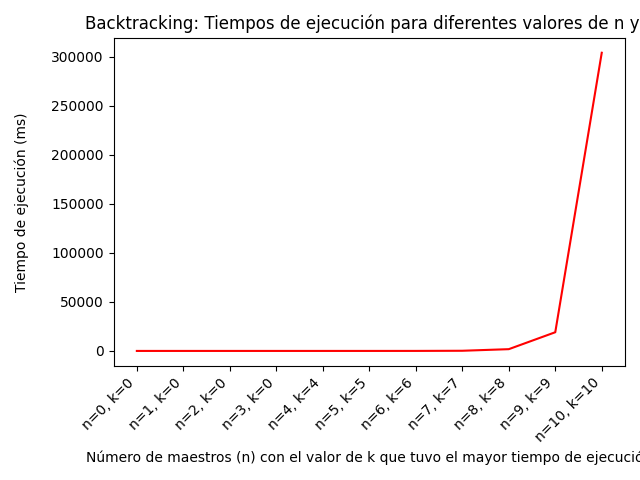
\includegraphics[scale=0.60]{images/graficoBacktracking.png}

Como podemos observar en la tendencia de la curva, el tiempo de ejecución aumenta exponencialmente con la cantidad de maestros $n$ y también depende de $k$. El tiempo más alto ocurre cuando $k$ se acerca a $n$, con $k < n$ (es lineal cuando $k = n$). Para valores pequeños de estas variables el algoritmo es relativamente rápido. Sin embargo, al incrementarlos no se vuelve práctico debido a que el tiempo no crece polinomialmente, sino exponencialmente.  Esto corrobora el análisis de la complejidad planteado previamente.

\subsubsection{Backtracking - greedy}
\label{sec:medidas-bt-greedy}
Procederemos a comparar esta versión del algoritmo de backtrcking con la anterior.

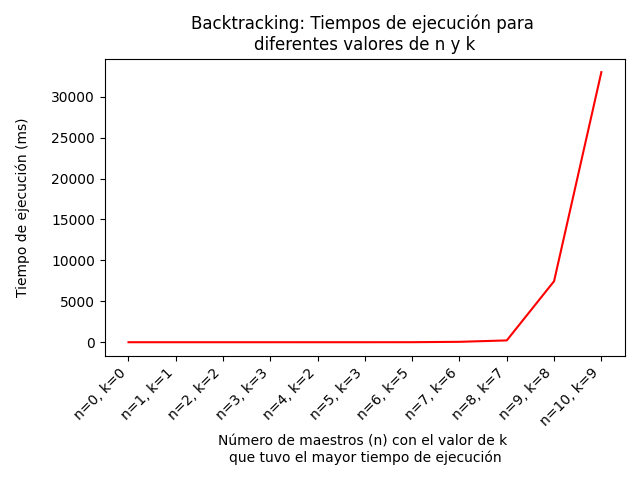
\includegraphics[scale=0.60]{images/graficoBacktrackingGreedy.png}

El gráfico evidencia una drástica disminución de los tiempos de ejecución, casi a la mitad de los del otro algoritmo. 

Nuevamente podemos observar la tendecia exponencial de la curva, que comprueba nuestra justificación de la complejidad temporal.

\subsection{Algoritmo de programación lineal}

Tomamos mediciones de tiempo con los mismos sets de datos utilizados para backtracking. Realizamos 2 gráficos para facilitar la comparación entre algoritmos. 

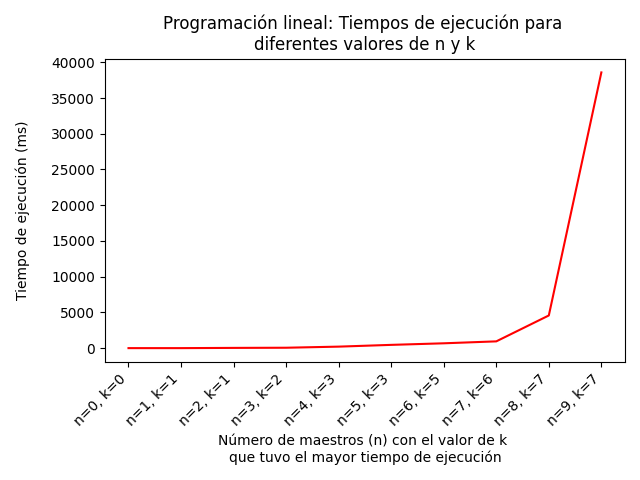
\includegraphics[scale=0.60]{images/graficoProgramacionLinealSin10.png}

El mejor algoritmo de backtracking tarda aproximadamente 35000 milisegundos en ejecutarse en el peor caso para $n = 10$. Sin embargo, PLE ya necesita 40000 milisegundos para $n = 9$. Esto es una gran diferencia con ambos algoritmos de backtracking que conllevan menos de 20000 milisegundos en ese caso.

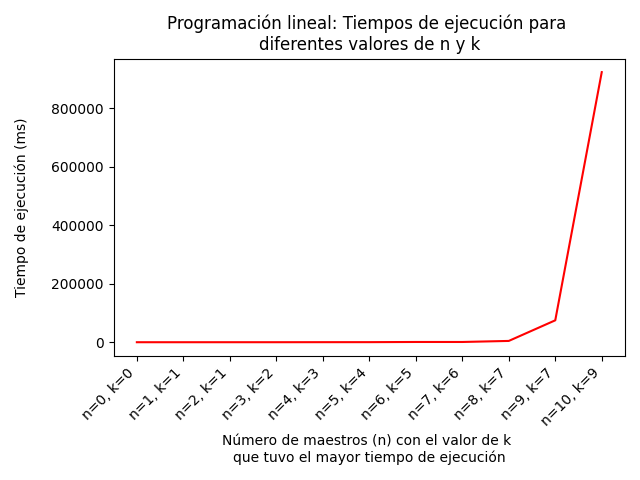
\includegraphics[scale=0.60]{images/graficoProgramacionLineal.png}

Analizando la totalidad de las mediciones, es evidente que nuestro algoritmo de programación lineal obtuvo tiempos de ejecución significativamente mayores a las dos implementaciones de backtracking. En todos los casos la complejidad temporal es exponencial, lo cual puede observarse en los respectivos gráficos. No obstante, para el conjunto de datos de entrada dado, el desempeño del algoritmo de PLE es peor.

\subsection{Algoritmos de Aproximación}
\subsubsection{Aproximación de la cátedra}
Realizamos mediciones con $n$ y $k$ hasta 1500 para corroborar la complejidad algorítmica de esta aproximación con valores inmanejables para el algoritmo exacto.

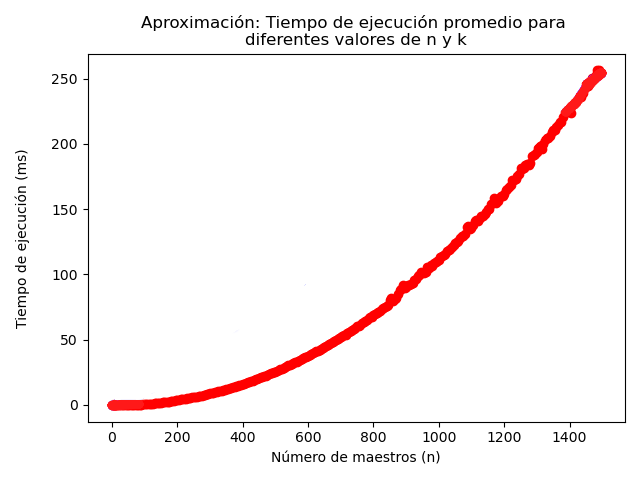
\includegraphics[scale=0.60]{images/graficoAproxCatedraReal.png}

Vemos que los puntos aparentan tomar la forma de una parábola no muy pronunciada. Lo cual refleja lo que obtuvimos en \nameref{sec:algoAproxCatedra}.
Si la complejidad del algoritmos fuese $\mathcal{O}(n \cdot n)$ veríamos una forma parabólica mas pronunciada, ya que la cantidad de maestros ($n$) suele ser considerablemente mayor que la cantidad de grupos ($k$). 
Sin embargo, como la complejidad del algoritmos es $\mathcal{O}(n \cdot k)$, la $k$ hace que la parábola tenga un crecimiento menos pronunciado.


\subsubsection{Aproximación adicional}

Realizamos mediciones con $n$ y $k$ hasta 1500 para corroborar la complejidad algorítmica de esta aproximación con valores inmanejables para el algoritmo exacto.

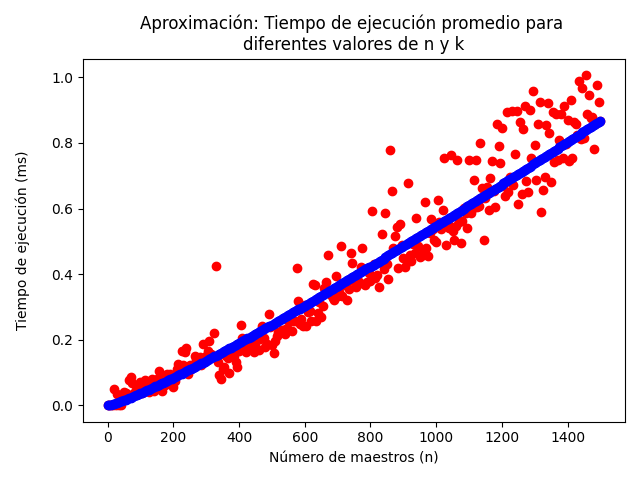
\includegraphics[scale=0.60]{images/graficoAproxAdicional.png}

Se puede observar una curva azul que representa $n \cdot \log(n)$, mientras que los puntos rojos son nuestras mediciones. 

También realizamos un gráfico con el set de datos usado en backtracking y programación lineal para mostrar la rapidez de este algoritmo en comparación con los exponenciales.

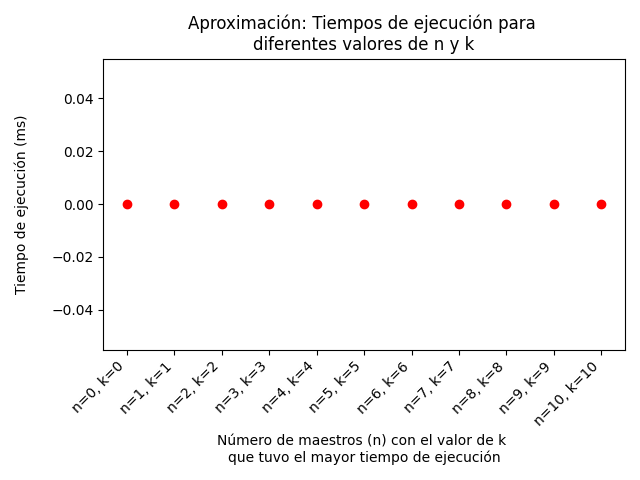
\includegraphics[scale=0.60]{images/graficoAproxAdicionalMediciones.png}

\section{Conclusión}

\end{document}
